\chapter{Indroduction to chaotic dynamics}
We begin with a few motivating examples.
\begin{ex}[Periodically forced slender beam]
	A beam is hanging on the inside of a rectangular frame, attached to the upper edge. Two permanent magnets are attached to the lower edge. Furthermore, there is a $T=2 \pi $-periodic forcing in the horizontal direction to the frame. The deflection of the beam is measured by the variable $x$. The setup is illustrated in Fig. \ref{fig:forced_slender_beam}.
	\begin{figure}[h!]
		\centering
		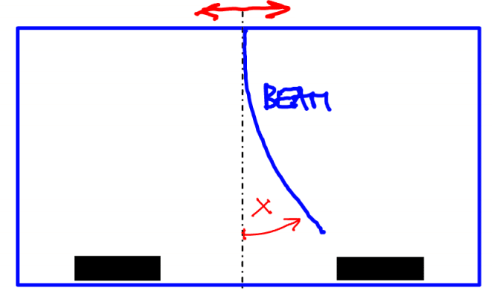
\includegraphics[width=0.5\textwidth]{figures/ch6/1forced_slender_beam.png}
		\caption{Depiction of the periodically forced slender beam. The frame is given by the blue rectangle. The two permanent magnets are represented by the black boxes.}
		\label{fig:forced_slender_beam}
	\end{figure}
This leads to the equation of motion
\begin{align}
	\ddot{x} + \dot{x} - x + x^3 = \varepsilon \cos(t);\quad 0 \leq \varepsilon \ll 1.
\end{align}
Therefore we have a perturbed Duffing oscillator. We transform the system into a first order ODE
\begin{align}
	\begin{dcases}
		\dot{x} = y \\
		\dot{y} = -y +x - x^3 + \varepsilon \cos(t).
	\end{dcases}
\end{align}
For $\varepsilon =0$ damping, two homoclinic orbits arise for the three fixed points. However, for nonzero damping, we get seemingly chaotic behavior. Both of these regimes are depicted in Fig. \ref{fig:pert_duffing}.
\begin{figure}[h!]
	\centering
	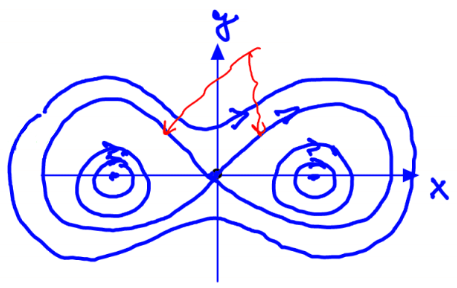
\includegraphics[width=0.45\textwidth]{figures/ch6/3unpert_duffing.png}
	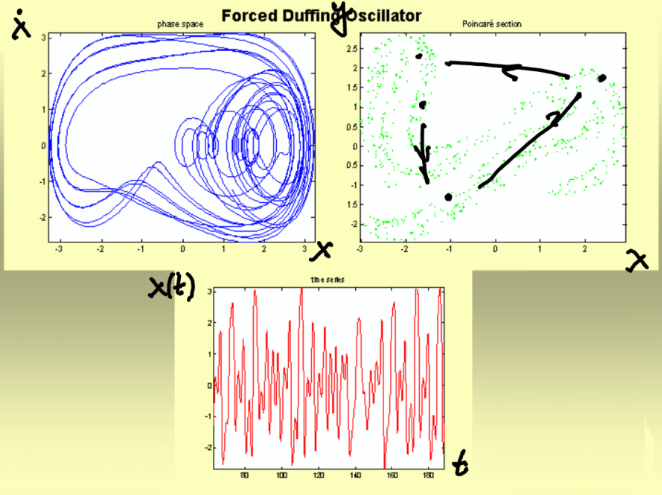
\includegraphics[width=0.45\textwidth]{figures/ch6/2pert_duffing.png}
	\caption{Left: Duffing oscillator with $\varepsilon=0$ damping, the red arrows designate the homoclinic orbits. Right: (Clockwise from top left) The phase space of the (nonzero) perturbed Duffing oscillator; The Poincaré section of the damped Duffing oscillator, with the Poincaré map illustrated by the black arrows; The value of $x(t)$ over time, with no apparent pattern.}
	\label{fig:pert_duffing}
\end{figure}

\end{ex}

\begin{ex}[2-dimensional Rayleigh-Bernard convection]
	A fluid is held between two plates. The upper plate is cold and the lower plate is hot. This causes convections to form as hotter fluid rises and colder fluid falls. So called convection cells then form for low Rayleigh numbers. This process is illustrated in Fig. \ref{fig:convection_cells}.
	\begin{figure}[h!]
		\centering
		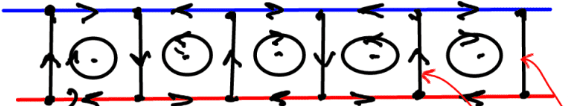
\includegraphics[width=0.65\textwidth]{figures/ch6/4convection_plates.png}
		\caption{Convection cells forming between two plates of different temperature. The cold plate (blue) is vertically above the hot plate (red). Each black dot represents a fixed point of the system, with heteroclinic orbits connecting them (red arrows). This is in an unperturbed setting ($\varepsilon =0 $).}
		\label{fig:convection_cells}
	\end{figure}

	If the Rayleigh number $R_{a}$ exceeds a critical value $R_{a_{ \textrm{crit} }}$, we have a time periodic perturbation to the velocity field. The fluid trajectories have the following equations of motion
	\begin{align}
		\begin{dcases}
			\dot{x} = u(x,y) + \varepsilon u_1(x,y,t) \\
			\dot{y} = v(x,y) + \varepsilon v_1 (x,y,t)
		\end{dcases}
;\quad \varepsilon>0.		
	\end{align}
	Here, the functions $u_1$ and $v_1$ are $T$-periodic. The chaotic nature of this system is shown in Fig. \ref{fig:convection_chaos}.
	\begin{figure}[h!]
		\centering
		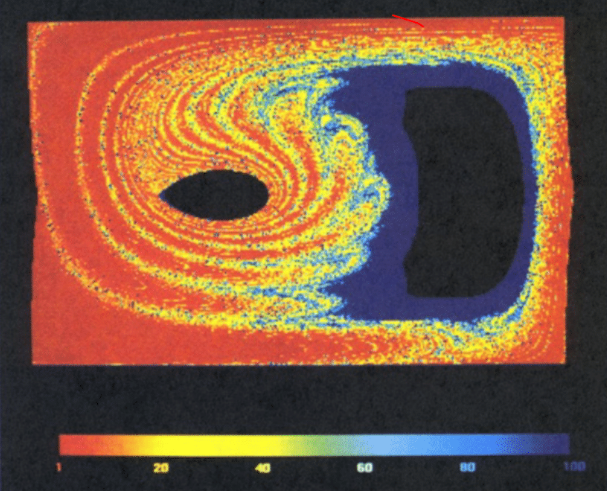
\includegraphics[width=0.4\textwidth]{figures/ch6/5convection_chaos.png}
		\caption{Escape time from one convection cell. The number of iterations of the Poincaré map needed for escape is given by the color scale. Here $0 < \varepsilon \leq 1$.}
		\label{fig:convection_chaos}
	\end{figure}
	
\end{ex}

Moving forward we will have a common mathematical setting
\begin{align}
	\dot{x} = f(x) + \varepsilon g(x,t);\quad x \in \mathbb{R}^{2},\quad g(x,t) =g(x,t+T);\quad 0 \leq \varepsilon \ll 1;\quad f,t\in C^{1}. \numberthis \label{eq7:one}
\end{align}
We have a small $T$-periodic perturbation of a planar ODE which can be studied via a Poincaré map $P_{\varepsilon}^{t_0}:x_0 \mapsto x(t_0 + T; t_0,x_0)$. Assume that for $\varepsilon=0$ the system \eqref{eq7:one} has a saddle type fixed point with a homoclinic (or heteroclinic) orbit $x^{0}(t-t_0)$. Such a system is depicted in Fig. \ref{fig:assumptions}.
\begin{figure}[h!]
	\centering
	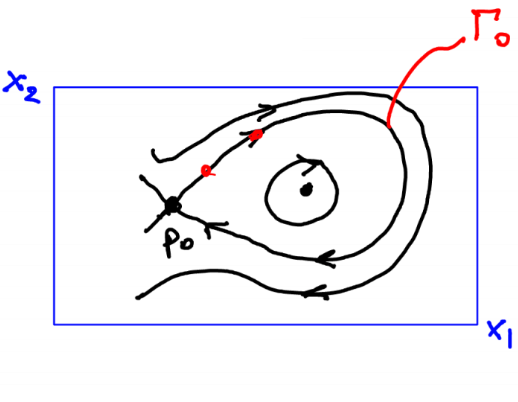
\includegraphics[width=0.45\textwidth]{figures/ch6/6assumptions_a.png}
	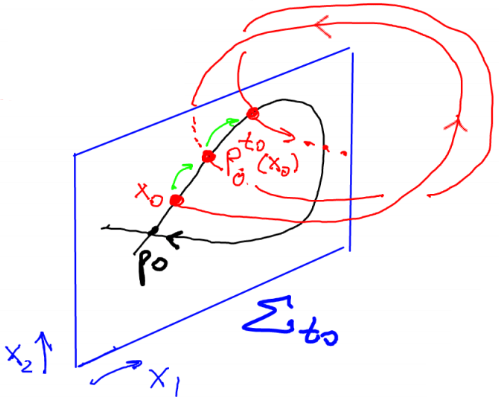
\includegraphics[width=0.45\textwidth]{figures/ch6/7assumptions_b.png}
	\caption{Left: An example of a system following the assumptions. The homoclinic orbit $\Gamma_0$ is equal to the local unstable and local stable manifolds. Right: The Poincaré map for $\varepsilon=0$, with time running counterclockwise about the $x_1$ axis with period $T$.}
	\label{fig:assumptions}
\end{figure}

\begin{remark}[]
	The fixed point of $P_{0}^{t_0}$ given by $p_0 $ is hyperbolic
	\begin{align}
	P_{0}^{t_0}(p_0) = p_0;\quad DP_{0}^{t_0}(p_0)  \textrm{ has eigenvalues }  \lambda_1,\lambda_2:\ |\lambda _1|<1,\ |\lambda _2|>1.
	\end{align}
	
\end{remark}

More generally we define a hyperbolic fixed point for a map.
\begin{definition}
	For a map $F:\mathbb{R}^{n}\to \mathbb{R}^{n}$ and a dynamical system with $x_{k+1} = F(x_k)$, the fixed point $p_0$ (i.e. $F(p_0) = p_0 $) is \emph{hyperbolic} if the linearization's $DF(p_0)\in \mathbb{R}^{n\times n}$ eigenvalues $\lambda_1,\ldots,\lambda_n $ never have unitary length: $|\lambda_i| \neq 1$ for $i=1,\ldots,n$.
\end{definition}

For each eigenvalue $\lambda _i$ of the linearization the corresponding eigenvector is given by $s_i$. Assume that $DF(p_0)$ is semisimple, i.e. all of the eigenvectors are linearly independent. The linearized dynamics at $p_0$ for $y=x-p_0$ small are
\begin{align}
	y_{k+1} = DF(p_0)y_k \implies y_k = \lambda_1^{k} c_1 s_1 + \ldots + \lambda_n^{k} c_n s_n.	
\end{align}
If all of the eigenvalues have less than unitary magnitude, $|\lambda _i|<1$ for $i=1,\ldots,n$, then $p_0$ is asymptotically stable. Otherwise if there exists an eigenvalue with norm strictly larger than 1, $p_0$ is unstable. The relationship of the nonlinear and linearized dynamics are shown in Fig. \ref{fig:lin_nonlin_relation}.
\begin{figure}[h!]
	\centering
	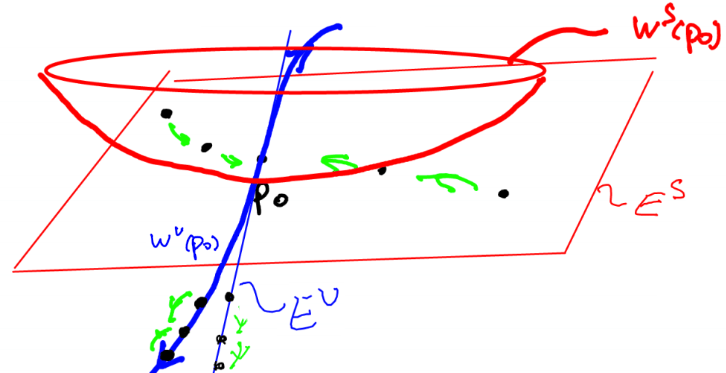
\includegraphics[width=0.65\textwidth]{figures/ch6/9lin_nonlin_relationship.png}
	\caption{The stable ($W^{S}(p_0)$) and unstable ($W^{U}(p_0)$) manifolds drawn in relation to the stable ($E^{S}$) and unstable ($E^{U}$) subspaces. The subspaces are given as the span of the stable (resp. unstable) eigenvectors. The green arrows signify steps of the linearized (resp. original) system.}
	\label{fig:lin_nonlin_relation}
\end{figure}

The fixed point $p_0$ along with the stable and unstable manifolds ($W^{S}(p_0)$ and $W^{U}(p_0)$) persist smoother under small smooth perturbations to $F$ near $p_0$.

\section{Consequences of hyperbolicity}
Hyperbolicity has a few important consequences in our setting. Foremost, the perturbed hyperbolic fixed point $p_{\varepsilon}^{t_0}$ has a hyperbolic periodic orbit for the ODE.Furthermore, the solutions of the ODE are smooth in $\varepsilon$, thus the solutions within $W^{U}(p_{\varepsilon}^{t_0})$ and $W^{S}(p_{\varepsilon}^{t_0})$ remain $\mathcal{O}(\varepsilon)$ close to $\Gamma_0$, i.e.

\begin{align}
	x_{\varepsilon}^{S}(t;t_0) &= x^{0}(t-t_0) + \varepsilon a^{S}(t) + \mathcal{O}(\varepsilon^{2} );\quad t\in [t_0,\infty ) \\
	x_{\varepsilon}^{U}(t;t_0) &= x^{0}(t-t_0) + \varepsilon a^{U}(t) + \mathcal{O}(\varepsilon^{2} );\quad t\in (-\infty, t_0].
\end{align}

Now we examine what the global shape of these manifolds are for $\varepsilon>0$ and if they interact. To do this we will follow an idea from Poincaré, Arnold, and Melnikov. To this end we define the perpendicular to $f$ 
\begin{align}
	f^{\perp}(x^{0}(0)) = 
	\begin{pmatrix}
		-f_2(x^{0}(0)) \\ f_1 (x^{0}(0))
	\end{pmatrix}
	.
\end{align}
We would like to use this to measure the distance between $x^{U}_{\varepsilon}(t_0;t_0)$ and $x^{S}_{\varepsilon}(t_0;t_0)$. The outlook for this is shown in Fig. \ref{fig:PAM_idea}.
\begin{figure}[h!]
	\centering
	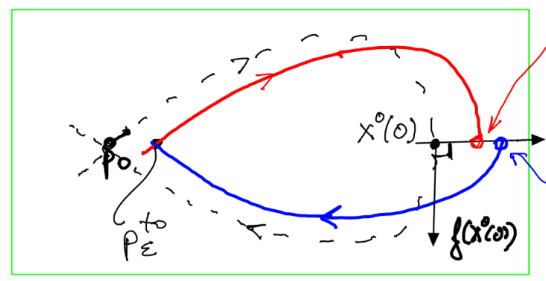
\includegraphics[width=0.5\textwidth]{figures/ch6/10PAM_idea.png}
	\caption{The Poincaré-Arnold-Melnikov idea. The dotted black line signifies $\Gamma$, the red dot $x^{U}_{\varepsilon}(t_0;t_0)$, the blue dot $x^{S}_{\varepsilon}(t_0;t_0)$, and the arrow pointing to the right $f^{\perp}$. The plane is $\Sigma_{t_0}$.}
	\label{fig:PAM_idea}
\end{figure}
Thus we have a signed distance function
\begin{align}
	d_{\varepsilon}(t_0) = \frac{\left\langle f^{\perp}(x^{0}(0)), x^{U}_{\varepsilon(t_0; t_0) - x^{S}_{\varepsilon}(t_0; t_0)}\right\rangle}{\left| f^{\perp}(x^{0}(0))\right|} 
	= \varepsilon  \frac{\left\langle f^{\perp}(x^{0}(0)), a^{U}(t_0) - a^{S}(t_0) \right\rangle}{\left| f^{\perp}(x^{0}(0))\right|} + \mathcal{O}(\varepsilon^2).
\end{align}
The numerator in the second equation is called the \emph{Melnikov function}
\begin{align}
	M(t_0)=\left\langle f^{\perp}(x^{0}(0)), a^{U}(t_0) - a^{S}(t_0) \right\rangle	.
\end{align}
In fact Melnikov proved an identity for this function.
\begin{theorem}[Melnikov]
	\begin{align}
		M(t_0) = \int_{-\infty }^{\infty }  \langle f^{\perp}(x^{0}(t-t_0)), g(x^{0}(t-t_0),t)\rangle dt.
	\end{align}
	For the proof, see the book by Guckenheimer \& Holmes.	
\end{theorem}
\begin{remark}[]
	The integral in Melnikov's theorem converges as $|g(x^{0}(t-t_0),t)|$ is globally bounded as $t \to \pm \infty $ and $|f^{\perp}| = |f|$ and
	\begin{align}
		\lim_{t\to \pm \infty }\left| f(x^{0}(t-t_0)) \right| =0,
	\end{align}
	exponentially as $p_0$ is a hyperbolic fixed point.	
\end{remark}

\begin{remark}[]
	In order to evaluate $M(t_0)$ we do not need to solve the perturbed ODE $\dot{x} =f(x) + \varepsilon g(x,t)$, instead we only need $x^{0}(t-t_0)$.
\end{remark}

Now observe that
\begin{align}
	d_{\varepsilon} (t_0) = 0 \iff \varepsilon \frac{M(t_0)}{\left| f^{\perp}(x^{0}(0))\right|} + \mathcal{O}(\varepsilon^2) = 0 \overset{\varepsilon \neq 0}{\iff} \underbrace{\frac{M(t_0)}{\left| f^{\perp}(x^{0}(0)) \right|} + \mathcal{O}(\varepsilon)=0}_{F(t_0, \varepsilon) = 0}.
\end{align}
Now we would like to know when we can find a solution $t_0(\varepsilon)$ such that $d_{\varepsilon}(t_0(\varepsilon))=0$ for $\varepsilon > 0$. To do this we use the Implicit Function Theorem. First assume that $F(\overline{t}_{0}, 0) = 0$, i.e. $M(\overline{t}_0) = 0$, and $\frac{\partial F}{\partial t_0}(\overline{t}_0), 0) \neq 0$, i.e. $\frac{\partial }{\partial t_0}M(\overline{t}_0) \neq 0$. If this condition is fulfilled the root is called \emph{transverse}.  Then there exists a unique $t_0(\varepsilon) = \overline{t}_{0} + \mathcal{O}(\varepsilon)$ which solves $F(t_0(\varepsilon), \varepsilon)=0$ for $\varepsilon \neq 0$ small enough. Also $t_0(\varepsilon)$ is smooth if $F(t_0,\cdot)$ is smooth.

A transverse zero for $M(t_0)$ implies that the Melnikov distance $d_{\varepsilon }(t_{0}(\varepsilon)=0$, in turn implying that the intersection of the stable and unstable manifolds have a nonzero intersection, $W^{S}(p_{\varepsilon}^{t_0}) \cap W^{U}(p_{\varepsilon}^{t_0}) \neq \emptyset$. Therefore we have an element $q\in W^{S}(p_{\varepsilon}^{t_0}) \cap W^{U}(p_{\varepsilon}^{t_0})$, for this $q$ we also have that for every $n \in \mathbb{Z}$
\begin{align}
	P_{\varepsilon}^{n}(q) \in W^{S}(p_{\varepsilon}^{t_0}) \cap W^{U}(p_{\varepsilon}^{t_0}). 
\end{align}
Therefore we have that for each iterate of the Poincaré map there is a unique point in both the stable and unstable manifolds, so these must intersect each other infinitely many times. This behavior is shown in Fig. \ref{fig:inf_intersections}. 
\begin{figure}[h!]
	\centering
	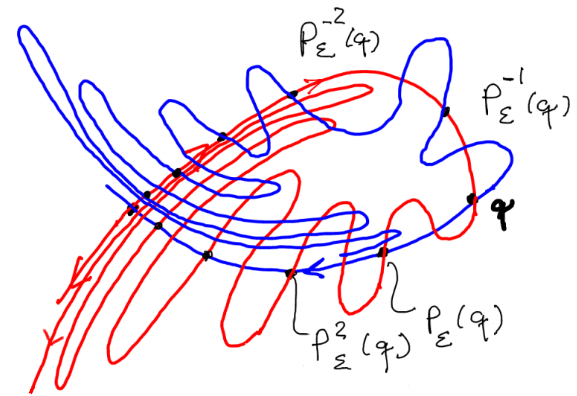
\includegraphics[width=0.45\textwidth]{figures/ch6/11inf_intersection_hetero.png}
	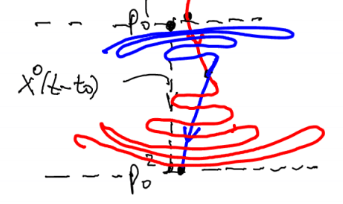
\includegraphics[width=0.45\textwidth]{figures/ch6/11inf_intersection_homo.png}
	\caption{The infinite intersections of the stable and unstable manifolds for a transitive zero. Left: The homoclinic case, this is aptly called a \emph{homoclinic tangle}. Right: The heteroclinic case.}
	\label{fig:inf_intersections}
\end{figure}
In the homoclinic tangle, we can see the accumulation of trajectories that are caused by the accumulation of the iterates of the Poincaré map. {\color{blue} He says to see the $\Lambda$ lemma, not sure exactly what is meant by that.}

\begin{remark}[]
	It is impossible for stable and unstable manifolds to intersect themselves. This is usually argued by stating that $q$ cannot have two distinctive preimages under a diffeomorphism. However, this is not sufficient as a self intersection does not imply that two distinct preimages exist, for instance a loop de loop manifold structure and suitable Poincaré map as in Fig. \ref{fig:loopdeloop}.
	\begin{figure}[h!]
		\centering
		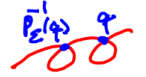
\includegraphics[width=0.25\textwidth]{figures/ch6/12loopdeloop.png}
		\caption{An example for a self-intersecting manifold without $q$ having multiple preimages.}
		\label{fig:loopdeloop}
	\end{figure}
A priori, this is possible to occur. In this case the existence of one loop actually implies the existence of infinitely many converging to $p_{\varepsilon}$. Thereby there must exist a loop in every arbitrarily small neighborhood of $p_{\varepsilon}$, this then contradicts the Hartman-Grobman Theorem as our system must be topologically equivalent to the linear saddle in a small enough neighborhood. 	
\end{remark}

\begin{remark}[]
	For every pair of intersections $P_{\varepsilon}^{k}(q)$ and $P _{\varepsilon}^{k+1}(q)$, there exists at least another intersection between the stable and unstable manifolds. This is due to the fact that $P_{\varepsilon}$ is orientation preserving (i.e. $DP_{\varepsilon}(q)$ is an orientation preserving linear map). The implication here is illustrated in Fig. \ref{fig:between_intersections}.
\begin{figure}[h!]
	\centering
	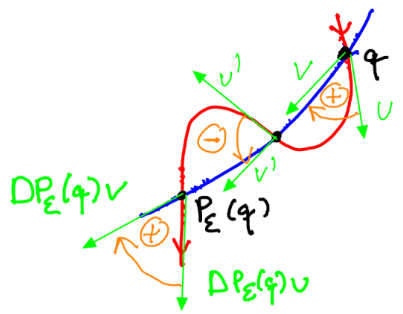
\includegraphics[width=0.5\textwidth]{figures/ch6/13between_intersections.png}
	\caption{Another intersection of the stable and unstable manifolds exists between two sequential iterates of the Poincaré map due to the preservation of orientation under this map.}
	\label{fig:between_intersections}
\end{figure}

The orientation preserving nature of $P_{\varepsilon}$ can be seen by using Liouville's Theorem 
	\begin{align}
		\det(DF_{t_0}^{t}(p)) = \exp \left( \int_{t_0}^{t}  \textrm{div}  ( f(x(s;t_0,p),s))ds\right),
	\end{align}
	for the flow map $F_{t_0}^{t}:x_0 \mapsto x(t;t_0,x_0)$	of the dynamical system $\dot{x} = f(x,t)$. In our case we find
	\begin{align}
		\det (DP_{\varepsilon}(q)) = \exp\left(\int_{t_0}^{t}  \textrm{div} \left. (f + \varepsilon g) \right|_{x_{\varepsilon}(t);\ x_{\varepsilon}(t_0)=q}) ds \right) > 0
	\end{align}
	Therefore $DP_{\varepsilon}(q)$ is orientation preserving, in fact Poincaré maps in general are orientation preserving.	
\end{remark}

\begin{ex}[The forced-damped Duffing equation]
Recall the dynamical system
\begin{align}
	\begin{dcases}
		\dot{x}=y \\
		\dot{y} = x - x^3  + \varepsilon ( \gamma \cos(\omega t) -\delta y)
	\end{dcases}
	;\quad |\varepsilon|\ll 1.
\end{align}
Here the forcing amplitude is given by $\gamma $ and the linear damping coefficient by $\delta $. We separate the right hand side into two parts
\begin{align}
	f(x,y) = 
	\begin{pmatrix}
		y \\ x - x^3
	\end{pmatrix},\quad
	g(x,y) =
	\begin{pmatrix}
	0 \\  \gamma \cos(\omega t) -\delta y
	\end{pmatrix}
	. \numberthis \label{eq7:juan}
\end{align}
A Hamiltonian for this system is given by 
\begin{align}
	H = \frac{1}{2}y^2 - \frac{1}{2} x^2  + \frac{1}{4}x^4 = E_{0} =  \textrm{const} .
\end{align}
Further the phase portrait for $\varepsilon=0$ is known and shown in Fig. \ref{fig:duffing_phase}. {\color{blue} He has $\varepsilon>0$ in the script, pg 12, but I think that is wrong.}
\begin{figure}[h!]
	\centering
	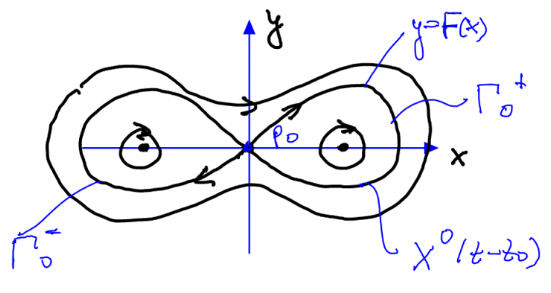
\includegraphics[width=0.5\textwidth]{figures/ch6/14duffing_phase.png}
	\caption{The phase portrait for the forced-damped Duffing oscillator for $\varepsilon=0.$}
	\label{fig:duffing_phase}
\end{figure}
We have that locally $\dot{x}=F(x)$, thus we have a separable equation. Colloquially this can be seen as follows (the implication is not rigorous and should not be interpreted as usual)
\begin{align}
	\frac{dx}{dt} = F(x) \implies \int_{0}^{x}  \frac{d \tilde{x}}{F(\tilde{x})} = \int_{0}^{t} d \tilde{t}.
\end{align}
Hence, on $\Gamma_{0}^{+}$, we have 
\begin{align}
	x_0(t) = 
	\begin{pmatrix}
		\sqrt{2}  \textrm{sech}(t) \\  -\sqrt{2}  \textrm{sech} (t) \tanh(t)
	\end{pmatrix}
.	
\end{align}
Now for $\varepsilon>0$ we calculate the Melnikov function
\begin{align}
	M^{+}(t_0) &= \int_{-\infty }^{\infty }\langle f^{\perp}(x^{0}(t-t_0), g(x^{0}(t-t_0), t) \rangle dt \\
		   &= - \frac{4 \delta }{3} + \sqrt{2} \gamma \pi \omega  \textrm{sech} \left( \frac{\pi \omega }{2}\right)\sin(\omega t_0). 
\end{align}
Next, we ask if this is equal to zero and look for a transverse zero. To this end we define $R^{0}(\omega) = \frac{4 \cosh \left( \frac{\pi \omega }{2}\right)}{3 \sqrt{2} \pi \omega }$. Thus the zeros of the Melnikov function are given by
 \begin{align}
	 R^{0}(\omega) = \frac{\gamma }{\delta} \sin(\omega t_0).
\end{align}
{\color{blue} I wasn't sure how he got the graph and what the marks meant, so I thought it wouldn't be clear to students, so I tried to do this part myself. I get the inverse result of him}.
A solution is then a transitive zero if the partial derivative with respect to $t_0$ is nontrivial
\begin{align}
	\sqrt{2} \gamma \pi  \omega ^2  \textrm{sech} \left( \frac{\pi \omega }{2}\right) \cos(\omega t_0) \neq 0
\end{align}
The $ \textrm{sech} $ function is nonzero, thus we only need to know when $\cos(\omega t_0)=0$, which occurs for $\omega t_0 = (2k+1)\pi $, or as a function of $t_0$ when $\frac{\omega }{\pi } = \frac{2k+1}{t_0}$. Thus at the odd integers scaled by $\frac{1}{t_0}$, we have nontransverse zeros, and all other roots of the Melnikov function are transverse. This is depicted in Fig. \ref{fig:beam_tangle}.
\begin{figure}[h!]
	\centering
	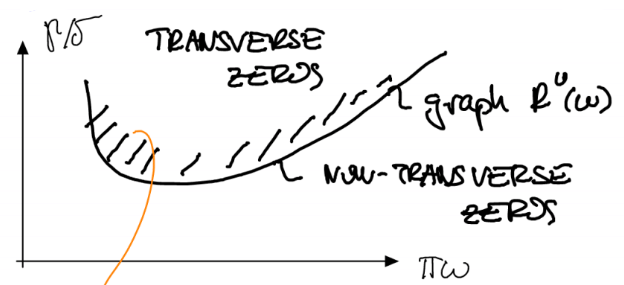
\includegraphics[width=0.6\textwidth]{figures/ch6/15beam_tangle.png}
	\caption{The yellow line showing that a homoclinic tangle exists for the forced-damped Duffing oscillator.}
	\label{fig:beam_tangle}
\end{figure}
{\color{blue} We need to go over this part I think.}
\end{ex}

\section{Dynamics near the homoclinic tangle \& Smale's horseshoe map}
We now continue and examine the dynamics near the homoclinic tangle. Consider the dynamical system
\begin{align}
	\dot{x} = f(x) + \varepsilon g(x,t);\quad x \in \mathbb{R}^{2};\quad f,g \in  \mathcal{C}^{1};\quad g(x,t) = g(x,t+T).
\end{align}
{\color{blue} Here I used mathcal\{C\} instead of C, I like this, think we should do it everywhere}
After an appropriate change of coordinates we find the geometry called \emph{Smale's construction}, which is as shown as in Fig. \ref{fig:smales_construction}.
\begin{figure}[h!]
	\centering
	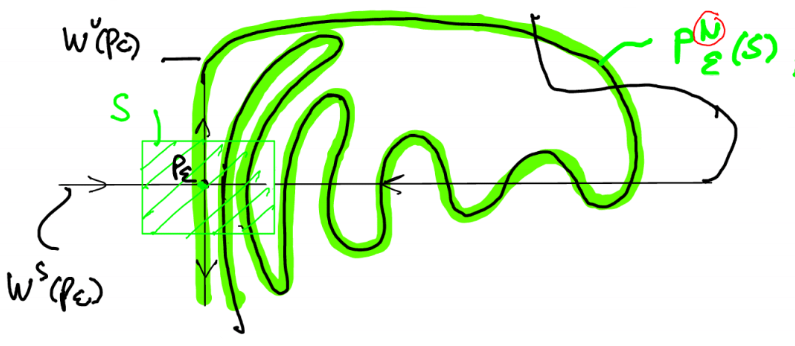
\includegraphics[width=0.7\textwidth]{figures/ch6/16smales_construction1.png}
	\hspace{0.03\textwidth}
	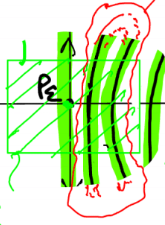
\includegraphics[width=0.25\textwidth]{figures/ch6/16smales_construction2.png}
	\caption{Smale's construction is found through an appropriate change of coordinates. Left: The full construction, the $N$ circled in red is large enough such that $P^{N}_{\varepsilon}(S)\cap S = \emptyset$, where $S$ is the green rectangle around $p_{\varepsilon}$. Right: Focus on the set $S$, the red lines designate a horseshoe-like structure.}
	\label{fig:smales_construction}
\end{figure}

A model for the right panel of Fig. \ref{fig:smales_construction} is given by \emph{Smale's Horseshoe map}. This is defined by first letting the set $S$ be equal to $[0,1]^2\in \mathbb{R}^{2}$, next the map itself is given by $f:S\to\mathbb{R}^{2}$. The map $f$ will not be defined explicitly, and instead geometrically. The unit square is divided into three horizontal strips, the upper one being labelled $H_2$ and the lower $H_1$. The square is then stretched vertically, and then smoothly bent to a horseshoe such that the previously upper horizontal strip now forms a vertical strip on the right side of the box $V_2$. Similarly, the lower horizontal strip now forms a vertical strip on the left $V_1$. Now the unit square can also be divided into three vertical strips, on the left $V_1$, an area in the middle, and on the right $V_2$. What was previously part of the middle horizontal strip now forms the connecting curve between $V_1$ and $V_2$. Furthermore, these vertical strips are straight, without any curvature on their boundary. The horseshoe map is depicted in Fig. \ref{fig:smale_map}. This map models the Poincaré map as seen before.
\begin{figure}[h!]
	\centering
	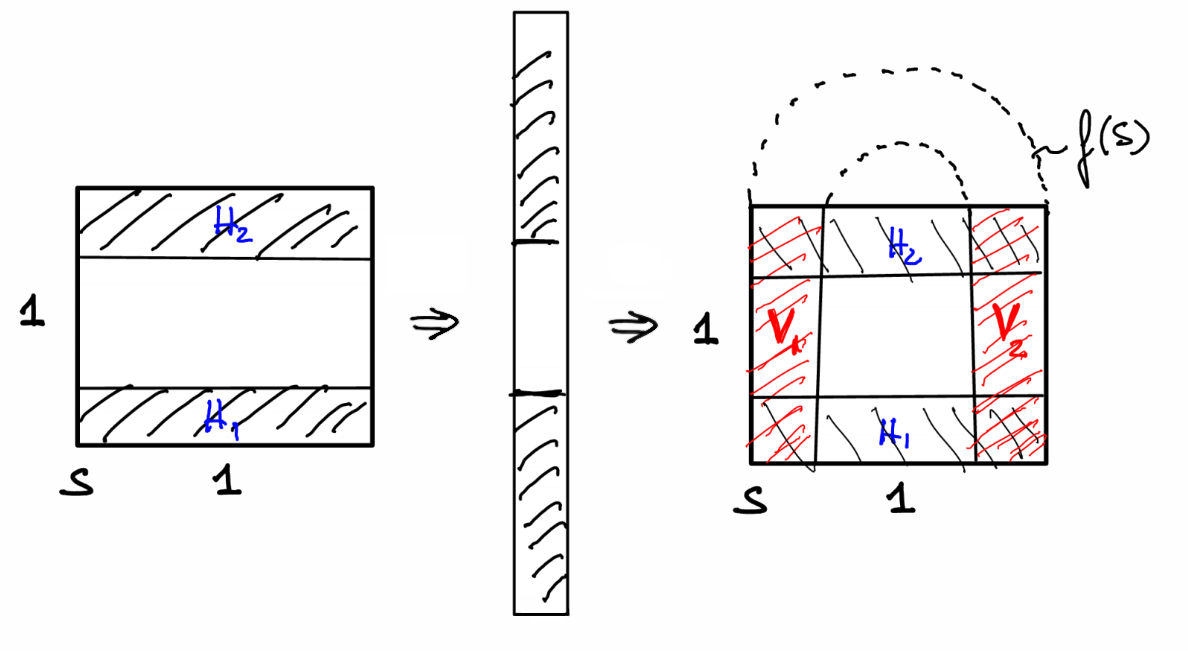
\includegraphics[width=0.8\textwidth]{figures/ch6/17smale_map.png}
	\caption{The two geometric steps of the Smale map, first a vertical stretch and then a fold into the horseshoe.}
	\label{fig:smale_map}
\end{figure}

Using this construction, we would like to know if any initial conditions stay in $S$ for long times (after many iterations of the Horseshoe map), despite the overall instability coming from $P_{\varepsilon}$. To further study this we introduce a couple definitions.
\begin{definition}
	The set of all points which stay in $S$ under $k$ backwards iterations is given by $V^{k}$.
\end{definition}
\begin{definition}[]
	For a map $f:X \to Y$, we denote the \emph{preimage} of a set $U\subset Y$ (or point $p\in Y$) as
	\begin{align}
		\boxed{
			f^{-1}(U) = \left\{ x\in X:\ f(x) \in U\right\}.
		}
	\end{align}
\end{definition}

 Under 1 backward iteration the set $V^{1}$ is given by the closed and nonempty set
	\begin{align}
		V^{1} = f \left( S \cap f^{-1}(S) \right) = f(S) \cap S = V_1 \cup V_2.
	\end{align}
For 2 backward iterations we have
\begin{align}
	V^{2} = f^{2}\left(S \cap f^{-1}(S) \cap f^{-2}(S) \right) = f^{2}(S) \cap f(S) \cap S  = V_{11} \cup V_{12} \cup V_{22} \cup V_{21} = \bigcup_{i_k \in \{1,2\}} V_{i_1i_2}.
\end{align}
The sets $V_{ij}$ are defined in Fig. \ref{fig:V_subsets}, the indices for each component are given by their orbit, those which after one iteration are in $V_i$ ($i\in\{1,2\}$) have the first index $i$, those which after two iterations are in $V_{j}$ have the second index $j$. Also the set $V^{2}$ is closed, nonempty, contained in $V^{1}$, and has $2^2$ components.
\begin{figure}[h!]
	\centering
	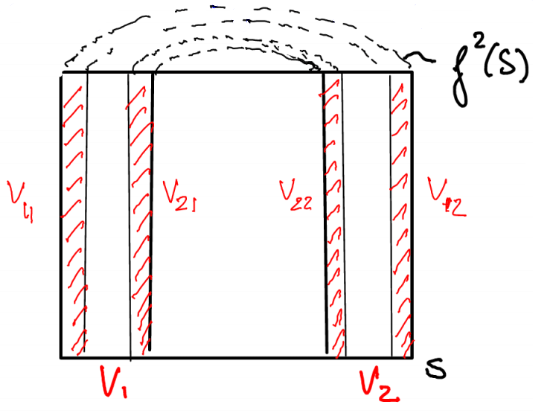
\includegraphics[width=0.35\textwidth]{figures/ch6/18V_subsets.png}
	\caption{The four components of $V^{2}$ with their index labels.}
	\label{fig:V_subsets}
\end{figure}

This continues for any number of backward iterates $k$ 
\begin{align}
	V^{k} = f^{k}\left(S \cap f^{-1}(S) \cap \ldots \cap f^{k}(S)\right) = f^{k}(S) \cap \ldots \cap f^{1}(S) \cap S = \bigcup_{i_j \in \{1,2\}}V_{i_1 \ldots i_k}.
\end{align}
This set has $2^k$ disjoint components (vertical strips) and is closed, nonempty, and contained in $V^{k-1}$. Therefore we have an infinite, nested sequence of nonempty and closed sets, therefore by Cantor's theorem we have 
\begin{align}
\boxed{
	V^{\infty } = \bigcap_{i=1}^{\infty } V^{i} \neq \emptyset.
}
\end{align}

\begin{remark}[]
	Cantor's theorem comes from the famous Cantor Dust which arises by first removing the open middle third of the unit interval in $\mathbb{R}$, and then iteratively removing the open middle third of each remaining interval. The Cantor Dust is a nonempty (in fact uncountably infinite) and disconnected set of points. For more on Cantor's theorem and Cantor's Dust, see any book on measure theory.
\end{remark}

\begin{definition}
	A set $U$ is called \emph{perfect} if it is closed and has no isolated points, i.e. given any point $x\in U$ and any distance $\varepsilon$ we can find a distinct element $y\in U$ such that $\|x-y\| < \varepsilon$.
\end{definition}
\begin{remark}[]
	This definition uses that the topology on $U$ was induced by a metric, which may not be the case in general, but is not relevant to the content here.
\end{remark}

In our case $V^{\infty }$ is in fact a Cantor set, i.e. it is a closed, nonempty set which is totally disconnected (the largest connected component is a line), and perfect.
{\color{blue} this set isn't totally disconnected, totally disconnected means that every connected subset is a singleton, here every connected set is a line. The projection of $V^{\infty}$ onto the unit interval in $\mathbb{R}$ is totally disconnected. We would need to define the quotient topology $S/\sim$ for $[x] =\left\{x+ \lambda 
	\begin{pmatrix}
		0 \\1
	\end{pmatrix}:\ \lambda \in [0,1] \right\}$ in order for each line to be a single element. I think this statement should apply to $\Lambda$, we should make that change and move this and the definition of perfect to after the definition of $\Lambda$.}

\begin{definition}
	Analogous to before we define the set of all points which stay in $S$ under $k$ forwards iterations is given by $H^{k}$. For each $k$ the set $H ^{k}$ is a nonempty set of $2^k$ closed, disjoint, horizontal strips, forming a nested sequence.
\end{definition}
By similar argumentation as before we have 
\begin{align}
	\boxed{
		H^{\infty } = \bigcap_{k=1}^{\infty} H^{k} \neq \emptyset.
	}
\end{align}

\begin{definition}
	The set of all points which stay in $S$ for all forward and backward iterates of the Smale Horseshoe map  is given by
	 \begin{align}
		\boxed{
\Lambda = H^{\infty } \cap V^{\infty }.
		}
	\end{align}
	The geometry of this set is shown in Fig. \ref{fig:lambda_def}.
	\begin{figure}[h!]
		\centering
		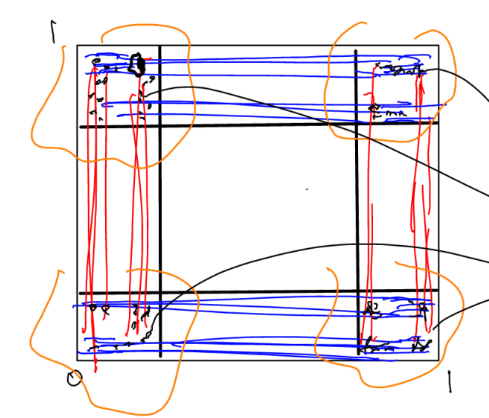
\includegraphics[width=0.4\textwidth]{figures/ch6/19lambda_def.png}
		\caption{The geometry of the set $\Lambda$, with the four regions containing points circled in orange. The red vertical lines represent the set $V^{\infty }$ and the blue horizontal lines the set $H^{\infty }$.}
		\label{fig:lambda_def}
	\end{figure}
\end{definition}

\begin{remark}[]
The set $\Lambda$ is a Cantor set of points.
\end{remark}

Returning to our case study of a Poincaré map with a homoclinic tangle, the points in $\Lambda$ keep coming back forever to the unstable periodic orbit as shown in Fig. \ref{fig:returning_points}. 
\begin{figure}[h!]
	\centering
	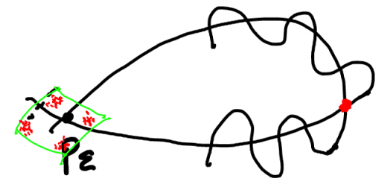
\includegraphics[width=0.3\textwidth]{figures/ch6/20returning_points.png}
	\caption{The homoclinic tangle with the set $S$ outlined in green and the elements of $\Lambda$ being denoted by the red dots within $S$.}
	\label{fig:returning_points}
\end{figure}

\section{Dynamics of Smale's Horseshoe map on the invariant set $\Lambda$}
We label any point $p\in \Lambda$ with an infinitely long binary sequence, which reflects the itinerary of $p$ in $\Lambda$ under iterations of $f$. For a given $p$, if we have 
\begin{align}
	\ldots,\
	f^{-2}(p) \in V_{s_{-3}},\
	f^{-1}(p) \in V_{s_{-2}},\
	p \in V_{s_{-1}},\
	p \in H_{s_{0}},\
	f^{}(p) \in H_{s_{1}},\
	f^{2}(p) \in H_{s_{2}},\
\ldots	
\end{align}
for $s_i\in \{1,2\}$ then we would have the itinerary 
\begin{align}
	\boxed{
s  = \ldots s_{-3}s_{-2}s_{-1} \bm{.}  s_0 s_{1}s_{2}\ldots.
	}
\end{align}
This is a unique symbolic encoding for \underline{all} points in $\Lambda$. Therefore $\Lambda$ is diffeomorphic to a space of doubly infinite sequences of two symbols. Such a space is just the space of outcomes for an infinite coin-tossing experiment. This equivalence of $\Lambda$ to the doubly infinite sequence of two symbols leads us to \emph{symbolic dynamics}: the analogue of the horseshoe map on the symbol space $\Sigma$.

In order to study these symbolic dynamics we need to know what the symbolic encoding of $f(p)$ is. For the analogue $\ldots s_{-2}s_{-1}\bm{.} s_0 s_1 s_2 \ldots = s\in \Sigma$ of $p\in \Lambda $, we can read off that $f(p)\in H_{s_1}$. Continuing in this fashion, we can see that $f(f(p))=f^{2}(p) \in H_{s_2}$ and so on, therefore $f(p)\in H^{\infty }$. By recalling that $f(H_{s_0}) = V_{s_0}$ we can see that $f(p) \in V_{s_0}$. Applying the definition of $f$ we find that $f^{-1}(f(p)) = p \in V_{s_{-1}}$. Therefore $f(p)\in V^{\infty }$ and thereby $f(p) \in \Lambda$. 

From our examination of the forward iterates of $f(p)$ we know that the symbolic encoding of $f(p)$ to the right of the dot is
\begin{align}
	\bm{.}s_1 s_2 s_3\ldots. 
\end{align}
Similarly, from our examination of the backwards iterates of $f(p)$ we know that the symbolic encoded of $f(p)$ to the left of the dot is
\begin{align}
\ldots s_{-2} s_{-1} s_{0} \bm{.}. 
\end{align}
Putting these together we get the symbolic encoding for $f(p)$ is 
\begin{align}
	\ldots s_{-2} s_{-1} s_{0} \bm{.} s_1 s_2 s_3 \ldots \in \Sigma.
\end{align}
So the encoding of $f(p)$ in the symbolic space is just a shift to the left on the encoding of $p$.

\begin{definition}
	We define the following three maps:
	\begin{enumerate}
		
\item The \emph{symbolic encoding map}
	\begin{align}
		\boxed{
			\phi:\Lambda \to \Sigma;\quad p \mapsto s= \phi(p);
		}
	\end{align}
	This map is a homeomorphism (i.e. it is continuous and has a continuous inverse).

\item The \emph{Smale Horseshoe map restricted to $\Lambda$}
	\begin{align}
		\boxed{
			\tilde{f}:\Lambda \to \Lambda;\quad p \mapsto f(p);
		}
	\end{align}
\item The \emph{Bernoulli shift map}
	\begin{align}
		\boxed{
			\sigma:\Sigma \to \Sigma;\quad
			\ldots s_{-2} s_{-1} \bm{.} s_0 s_1 s_2 \ldots 
			\mapsto
			\ldots s_{-2}s_{-1}s_{0}\bm{.} s_1 s_2 s_3 \ldots.
		}
	\end{align}
	
	\end{enumerate}
\end{definition}
We have that the following diagram commutes
\begin{equation}
\begin{tikzcd}
	\Sigma \arrow[r, "\sigma"] 
& \Sigma \\
\Lambda \arrow[u,"\phi"] \arrow[r, "\tilde{f}"]
& \Lambda \arrow[u, "\phi"] 
\end{tikzcd}.
\end{equation}
Therefore $\tilde{f} = \left. f\right|_{\Lambda}$ is topologically conjugate to a Bernoulli shift on $\Sigma$ 
	\begin{align}
		f = \phi^{-1} \circ \sigma \circ \phi.
	\end{align}
Hence, orbits of $f$ are taken to those of $\sigma$, with their orientation preserved.	
